\section{Iteración V}
\subsection{Resumen}
En esta iteración desarrollamos la función \textbf{ARFRecoverAccount} para implementar un proceso seguro de recuperación de la contraseña de una cuenta en caso de haberla olvidado.

\subsection{Desarrollo}
El método cumple la regla de negocio \textbf{BR3} y sigue el proceso de negocios mostrado en la figura x.xx. A nivel aplicativo consta de tres pasos, cada uno con sus respectiva pantalla:
\begin{itemize}
	\item El usuario ingresa el email de su cuenta de la cual quiere recuperar la contraseña (ver figura x.xx)
	\item El sistema genera y envía un código al email de la cuenta. El usuario deberá escribir este código en la aplicación para verificar que tiene acceso al correo y así validar que efectivamente sea su cuenta (ver figura x.x).
	\item El usuario escribe una nueva contraseña y la guarda para sustituir a la contraseña anterior (ver figura x.x).
\end{itemize}
\begin{figure}[h!]
	\centering
	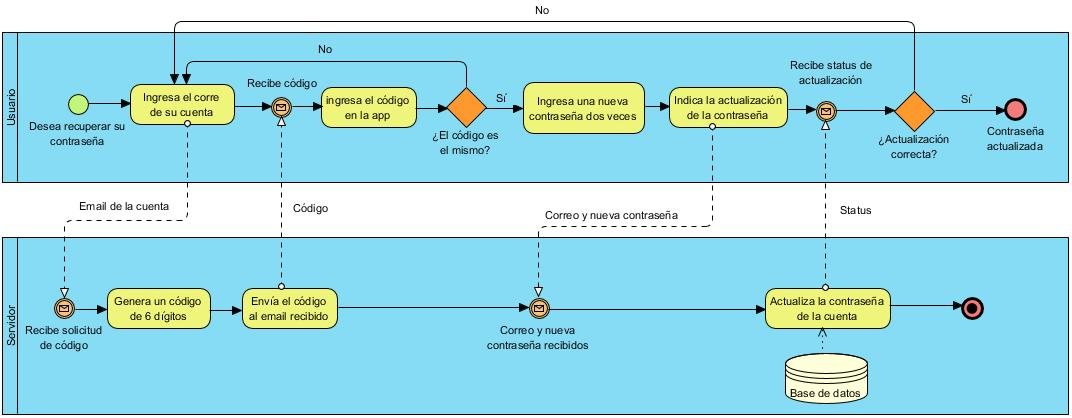
\includegraphics[width=15cm,height=6cm]{imagenes/desarrollo/diagramas/BPMN_RECOVER.jpg}
	\caption{Diagrama de proceso de recuperación de contraseña.}
	\label{fig:recover}
\end{figure}
